\mysubsection{Commande Angulaire et Cartésienne}\label{Comm_Ang_e_Cart}
Avant de commencer à développer le système de commande pour le robot, on doit comprendre son modèle dynamique. L'idée principale est de contrôler la position de l'outil du robot par le couple mécanique développer dans chaque articulation. Alors, la relation entre ces deux grandeurs, avec la position de l'outil décrite comme des angles de chaque articulation du robot, est le modèle dynamique direct:


	\begin{equation}
		\bm{\Gamma} = \bm{A}(\bm{q})*\ddot{\bm{q}}+\bm{H}(\bm{q},\dot{\bm{q}})
	\end{equation}

D'où $ \bm{\Gamma} $ le vecteur des couples nécessaires dans chaque articulation du robot, q le vecteur des positions angulaires de chaque articulation du robot, $ \bm{A}(\bm{q}) $ la matrice d'inertie du robot et $ \bm{H}(\bm{q},\dot{\bm{q}}) $ les couples dissipatives du robot (Coriollis, friction et gravitationnel).

Pour mettre en œuvre le système de commande du robot, on se basera sur l'équation précédent et on développera les lois de commande premièrement dans l'espace des articulations et ensuite dans l'espace opérationnel.
\subsubsection{Commande Angulaire}\label{Comm_Ang}

On commencera pour la commande du robot dans l'espace des articulations pour deux raisons différentes: il est plus facile d'être mis en oeuvre, alors on développe le projet dans un ordre de difficulté croissant; on n'a pas besoin de relations intermédiaires pour convertir du modèle angulaire au modèle opérationnel (modèle géométrique direct plus jacobien), donc la performance obtenu est due uniquement au système de commande et on peut l'optimiser et l'utiliser comme base pour générer le système de commande dans l'espace opérationnel. On a utilisé deux approches différentes pour générer les lois de commande pour le robot, et on a les comparé pour choisir le plus efficace.

Dans la première approche, il s'agit de considérer que chaque articulation du robot est découplé des autres. Donc on peut écrire pour chaque articulation:

\begin{equation}
	\Gamma_i =  a_i*\ddot{q}_i+Fv_i*\dot{q}_i+\gamma_i
\end{equation}

D'où $ a_i $ est la magnitute maximale de l'élément (i,i)  de la matrice d'inertie, $ Fv_i $ est le coefficient de friction par rapport à l'articulation i et $ \gamma_i $ est une perturbation (due, par exemple, au couple gravitationnel).

Si on a le modèle dynamique du robot, on peut trouver les paramètres précédents et contrôler séparément chaque articulation du robot en utilisant un PID par exemple. Dans ce cas, la fonction de transfert qu'on obtiendra entre la position de référence et la vraie position du robot pour chaque articulation est:


	\begin{equation}
		 H_i(s) = \frac{Kd_is^2 + Kp_is + Ki_i}{a_is^3 + (Kd_i + Fv_i)s^2 + Kp_is + Ki_i}
	\end{equation}

Alors, l'équation caractéristique est $ d(s)$ = $a_is^3 + (Kd_i + Fv_i)s^2 + Kp_is + Ki_i $, et on peut choisir $ Kp $, $ Ki $ e $ Kd $ pour déterminer la dynamique du robot en boucle fermée. On veut que le dépassement de la réponse indicielle soit nulle, alors on a besoin que $ d(s)$ = $ a_i(s + \omega_i)^3 $, $ \omega $ choisi de façon à contrôler le temps de réponse du système. Cependant, il y a un compromis dans le choix de $ \omega $, parce que s'il est petit, le système sera trop lent, mais s'il est trop gros, on peut arriver à la fréquence de résonance du système. Alors, on peut calculer $ Kp $, $ Ki $ et $ Kd $ selon les formules suivantes. On a aussi le schéma de commande du robot obtenu sur simulink.

	\begin{subequations}
	\begin{equation}
		Kp_i = 3a_i(\omega_i)^2
	\end{equation}
	\begin{equation}
	Kd_i = 3a_i(\omega_i) - Fv_i\\
	\end{equation}
	\begin{equation}
	Ki_i = a_i(\omega_i)^3
	\end{equation}
	\end{subequations}

%\todo{formula: Kp_i = 3*a_i*(omega_i)^2}\\
%\todo{formula: Kd_i = 3*a_i*omega_i - Fv_i)}\\
%\todo{formula: Kp_i = a_i*(omega_i)^3}

\begin{figure}[H]
	\begin{center}	
		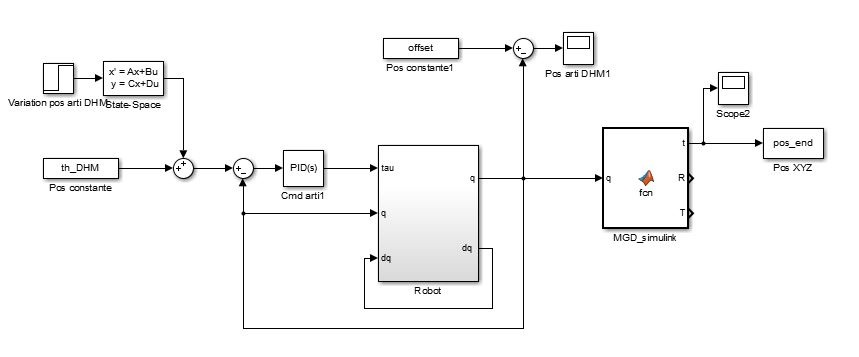
\includegraphics[width=\textwidth]{./PID_joint_space_diagram.JPG}
		\caption{Schéma de commande angulaire PID}
		\label{fig:PID_joint_space_diagram}
	\end{center}
\end{figure}
%\todo{figura: PID joint space diagram}
%\todo{legenda da figura: }

La deuxième approche de commande pour le robot est la technique de compensation des non-linéarités. Il s'agit d'utiliser la matrice d'inertie $ \bm{\hat{A}}(\bm{q}) $ et le vecteur des couples 
$ \hat{\bm{H}}(\bm{q},\dot{\bm{q}}) $ estimées pour déterminer le couple nécessaire pour le robot. Alors, on utilisera la relation:


	\begin{equation}
		\bm{\Gamma} = \bm{\hat{A}}(\bm{q})*\bm{w}(t) + \hat{\bm{H}}(\bm{q},\dot{\bm{q}})
	\end{equation}

Si $  \bm{\hat{A}} $ et $ \hat{\bm{H}} $ modélisent bien le modèle dynamique du robot, on peut choisir $ \bm{w}(t) = \ddot{\bm{q}} $ et cela correspond exactement au modèle dynamique direct du robot. Avec cette approche, on peut calculer le couple nécessaire avant de l'alimenter dans le robot et de cette façon on peut réduire les fluctuations dans la réponse dues aux non-linéarité du modèle du robot. Cette technique rend plus facile aussi pour mettre en oeuvre la loi de commande. On définit l'erreur de position comme la différence entre la position désirée et la vraie position du robot ($ \bm{e} = \bm{q_d} - \bm{q} $), et si on utilise un PID pour le contrôleur:


	\begin{equation}
		\bm{w}(t) = \ddot{\bm{q}}_d+ \bm{Kp}(\bm{q}_d- \bm{q}) + \bm{Kd}(\dot{\bm{q}}_d - \dot{\bm{q}}) + \bm{Ki}\int_0^t (\bm{q}_d - \bm{q})d\tau = \ddot{\bm{q}}
	\end{equation}
	
	
avec $ \bm{Kp} $, $ \bm{Kd} $ et $ \bm{Ki} $ matrices diagonales.

On peut développer dans le domaine de Laplace: 
\begin{subequations}
\begin{equation*}
\bm{w}(t)  =  \ddot{\bm{q}}_d + \bm{Kp}(\bm{q}_d- \bm{q}) + \bm{Kd}(\dot{\bm{q}}_d - \dot{\bm{q}}) + \bm{Ki}\int_0^t (\bm{q}_d - \bm{q})d\tau 
\end{equation*} 
\begin{equation*}
 s^3\bm{E}(s)+ s^2\bm{Kd}*\bm{E}(s) +s*\bm{Kp}*\bm{E}(s) + \bm{Ki}*\bm{E}(s)=  s^2*\bm{e}(0)+ s*\bm{e}(0) +\bm{e}(0)
\end{equation*} 
\end{subequations} 
%\todo{formula: s^3*vect(E(s)) + vect(Kd)*s^2*vect(E(s)) + vect(Kp)*s*vect(E(s)) + vect(Ki)*vect(E(s)) = s^2*vect(e(0)) + s*(vect(e(0)) + vect(e.(0)))}


Alors, pour chaque articulation $ E_i(s) $ = $ \dfrac{s^2*e_i(0) + s*(e_i(0) + \dot{e}_i(0))}{s^3 + Kd_i*s^2 + Kp_i*s + Ki_i} $ 
%\todo{formula: E_i(s) = (s^2*e_i(0) + s*(e_i(0) + e._i(0)))/(s^3 + Kd_i*s^2 + Kp_i*s + Ki_i)}

Comme il a été dit, on veut que le dépassement de la réponse indicielle soit nulle, et pour une pulsation de brisure $ \omega_i $, on a:

\begin{subequations}
	\begin{equation}
		Kp_i = 3\omega_i^2
	\end{equation}
	\begin{equation}
		Kd_i = 3\omega_i
	\end{equation}
	\begin{equation}
		Ki_i = \omega_i^3
	\end{equation}
\end{subequations}


%\todo{formula: Kp_i = 3*(omega_i)^2}
%\todo{formula: Kd_i = 3*omega_i}
%\todo{formula: Kp_i = (omega_i)^3}

Dans la figure suivante, on a le schéma de cette approche de commande angulaire qu'on a mis en oeuvre sur Simulink. Par rapport à la technique de commande du PID, on peut noter que cette technique permet, en plus, de fournir des consignes de vitesse et accélération et pas seulement de position, ce qui est nécessaire pour que le robot puisse suivre des trajectoires.
\begin{figure}[H]
	\begin{center}	
		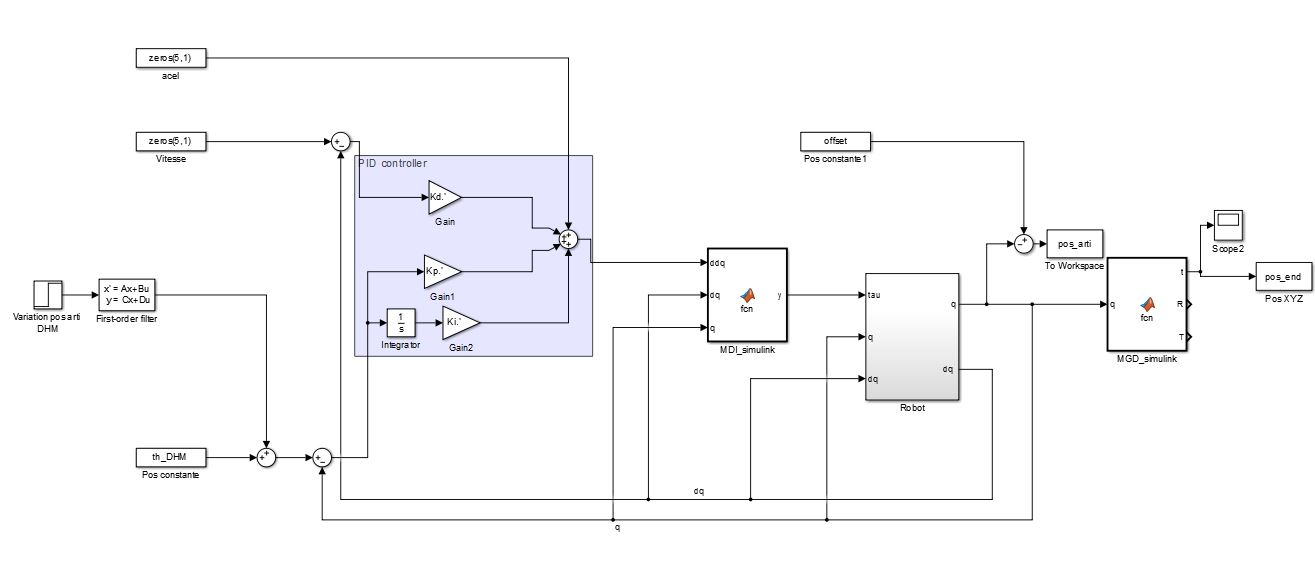
\includegraphics[width=\textwidth]{./CTI_joint_space_diagram.JPG}
		\caption{Schéma de commande angulaire PID avec compensation des non-linéarités}
		\label{fig:CTI_joint_space_diagram}
	\end{center}
\end{figure}
%\todo{figura: CTI joint space diagram}
%\todo{legenda da figura: Schéma de commande angulaire PID avec compensation des non-linéarités}
\subsubsection{Commande Cartésienne}\label{Comm_Cart}

Pour mettre en oeuvre les lois de commande du robot dans l'espace opérationnel, on utilisera les mêmes deux approches précédentes. La différence ici est qu'on doit utiliser des fonctions pour convertir les informations de l'espace angulaire à l'espace opérationnel. Cela peut être faite en utilisant le Jacobien. 

Premièrement, pour obtenir les informations cartésiennes de la position de l'outil du robot avec les positions angulaires des articulations on doit utiliser le modèle géométrique directe du robot. Ce modèle est basé sur des changements de repère: on définit un repère dans chaque articulation du robot, un dans la base et un autre dans l'outil. L'idée est de créer une matrice homogène de transformation de repère (position et direction) d'une articulation par rapport à l'articulation précédente, qui dépend des paramètres constructifs du robot et des angles des articulations. Pour multiplier ces matrices, on peut obtenir la position et orientation de l'outil du robot par rapport au repère dans la base du robot comme fonction des angles des articulations. Pour obtenir la vitesse cartésienne de l'outil, on peut utiliser directement le Jacobien, selon la relation:

\begin{equation}
	\dot{\bm{X}}=\bm{J}\dot{\bm{q}}
\end{equation}

%\todo{fórmula: vect(X.) = mat(J)*vect(q.)}

D'où $ \bm{X} $ est la position de l'outil du robot dans l'espace opérationnel et J est le Jacobien.

Pour générer le couple nécessaire pour le robot avec des erreurs de position cartésienne, on peut utiliser le Jacobien transposée, et l'équation du PID devient maintenant:

	\begin{equation}
	\bm{\Gamma} = \bm{J}^T\left[\bm{Kp}(\bm{X}_d - \bm{X})+\bm{Kd}(\dot{\bm{X}}_d - \dot{\bm{X}}) +\bm{Ki}\int_0^t(\bm{X}_d - \bm{X})d\tau\right]
	\end{equation}

%\todo{fórmula: vect(gamma) = mat(transpose(J))*[vect(Kp)*(vect(X_d) - vect(X)) + vect(Kd)*(vect(X._d) - vect(X.)) + vect(Ki)*integral(de 0 a t)(vect(X_d) - vect(X))dtau ]}

avec $ \bm{Kp} $, $ \bm{Kd} $ et $ \bm{Ki} $ matrices diagonales.

Dans cette nouvelle configuration, l'équation qui relie la position désirée et la vraie position du robot n'est plus découplé, alors il est très compliqué de définir analytiquement les paramètres $ \bm{Kp} $, $ \bm{Kd} $  et $ \bm{Ki} $ du contrôleur. Ce qu'on sait est que le terme intégral agit sur l'élimination de l'erreur statique, mais il réduit la stabilité du système, alors on peut définir un temps acceptable pour éliminer les perturbations en échelon et choisir le $ \bm{Ki} $; le terme dérivatif est un terme prédictive, alors il agit en réduisant le dépassement de la réponse; et le terme proportionnel est liée à l'intensité de l'action de contrôle par rapport à l'erreur, alors il peut régler la vitesse de réponse. Avec ses informations et les spécifications du système, on peut régler manuellement les paramètres $ \bm{Kd} $ et $ \bm{Kp} $. Mais on doit prendre en considération aussi que, si $ \bm{Kd} $ et $ \bm{Kp} $ sont trop gros, le système peut devenir instable.

Le schéma de commande pour le système est montré dans la figure suivante, générer avec le logiciel Simulink.

\begin{figure}[H]
	\begin{center}	
		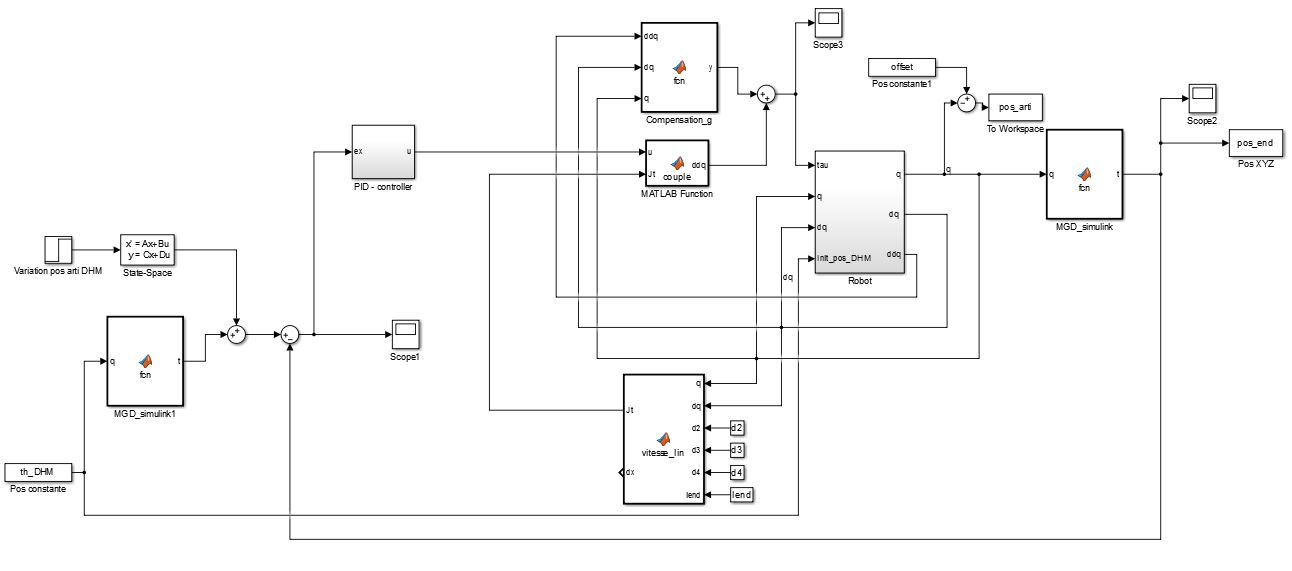
\includegraphics[width=\textwidth]{./PID_operational_space_diagram.JPG}
		\caption{Schéma de commande cartésienne PID}
		\label{fig:PID_operational_space_diagram}
	\end{center}
\end{figure}
%\todo{figura: PID operational space diagram}
%\todo{legenda da figura: Schéma de commande cartésienne PID}

On peut utiliser les mêmes principes précédents pour générer la loi de commande dans l'espace opérationnel avec la technique de compensation des non-linéarités, sauf que la relation entre le couple et l'erreur de position cartésienne devient:

\begin{equation}
	\bm{\Gamma} = \bm{\hat{A}}\bm{J^{-1}}(\bm{w}(t) - \bm{\dot{J}}*\dot{\bm{q}}) + \hat{\bm{H}}
\end{equation}

%\todo{formula: vect(Gama) = Mat(Â)*Mat(J^-1)*(vect(w(t)) - Mat(J.)*vect(q.)) + vect(^H)}

Si le modèle du robot est bon, on aura $ \bm{w}(t)$ = $ \dot{\bm{X}} $
%\todo{formula: vect(w(t)) = vect(X.)}
, et comme dans le cas équivalent dans l'espace des articulations, on peut écrire, si on utilise un contrôleur PID, et avec $ \bm{e}_x $ = $ \bm{X}_d - \bm{X} $
%\todo{vect(e_x) = vect(X_d) - vect(X)}
:

\begin{equation}
	E_{x_i}(s)= \frac{s^2*e_{x_i}(0) + s*(e_{x_i}(0) + \dot{e}_{x_i}(0))}{s^3 + Kd_i*s^2 + Kp_i*s + Ki_i}
\end{equation}

%\todo{formula: E_x_i(s) = (s^2*e_x_i(0) + s*(e_x_i(0) + e._x_i(0)))/(s^3 + Kd_i*s^2 + Kp_i*s + Ki_i)}

Comme on veut que le dépassement de la réponse indicielle soit nulle, et pour une pulsation de brisure $ \omega_i $
%\todo{\omega_i}
 choisi maintenant pour la position et orientation de l'outil, on a à nouveau:

\begin{subequations}
	\begin{equation}
		Kp_i = 3\omega_i^2
	\end{equation}
	\begin{equation}
		Kd_i = 3\omega_i
	\end{equation}
	\begin{equation}
		Ki_i = \omega_i^3
	\end{equation}
\end{subequations}
%\todo{formula: Kp_i = 3*(omega_i)^2}
%\todo{formula: Kd_i = 3*omega_i}
%\todo{formula: Kp_i = (omega_i)^3}

Le schéma de commande pour le système est montré dans la figure suivante, générer avec le logiciel Simulink.

\begin{figure}[H]
	\begin{center}	
		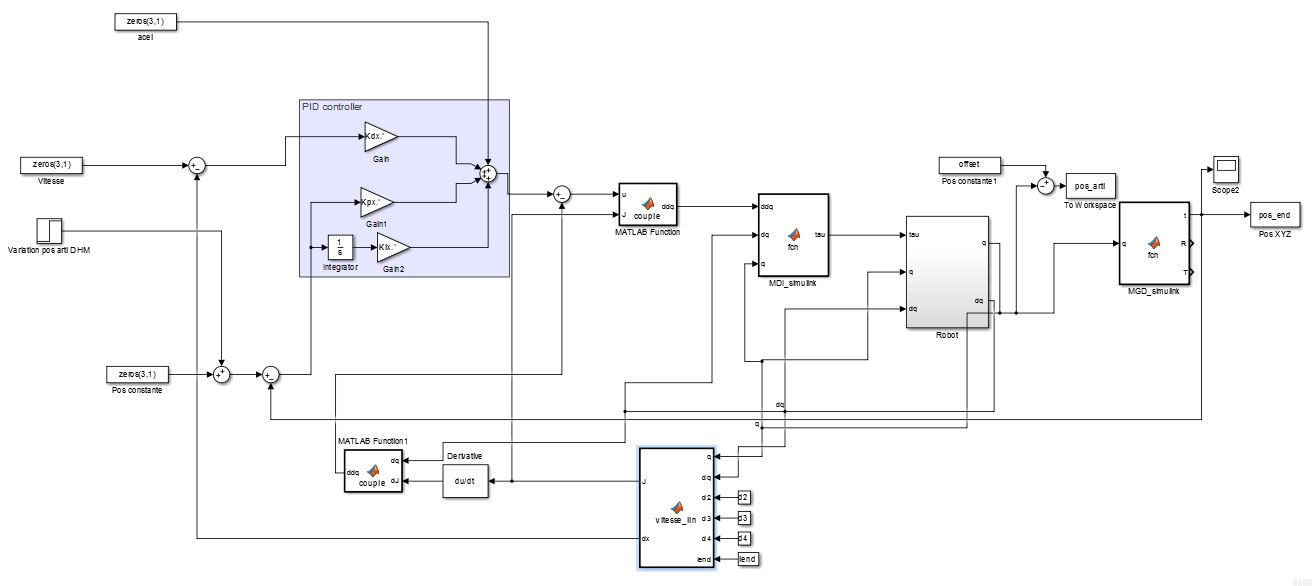
\includegraphics[width=\textwidth]{./CTI_operational_space_diagram.JPG}
		\caption{Schéma de commande cartésienne PID avec compensation des non-linéarités}
		\label{fig:CTI_operational_space_diagram}
	\end{center}
\end{figure}
%\todo{figura: CTI operational space diagram}
%\todo{legenda da figura: Schéma de commande cartésienne PID avec compensation des non-linéarités}